\subsection{Traitement du texte avec CamemBERT}

Pour parvenir à détecter le changement de tour de parole dans les données textuelles, nous avons choisi d'utiliser un modèle
considéré comme l'état de l'art pour la tâche de classification de texte : le modèle BERT (Bidirectional Encoder
Representations from Transformers~\cite{Bert}). Ce modèle utilise notament les Transformers~\cite{transformers} 
(voir son architecture Figure~\ref{fig: Transformers}).

Par ailleurs, BERT étant un modèle comprenant un nombre important de paramètres (environ 100 millions) il est inenvisageable avec
nos moyens de l'entraîner "à partir de 0". Nous avons donc opté pour l'utilisation d'un modèle pré-entrainé sur la langue Française
appelé CamemBERT et nous avons gelé les poids de CamemBERT.

\begin{figure}[H]
    \centering
    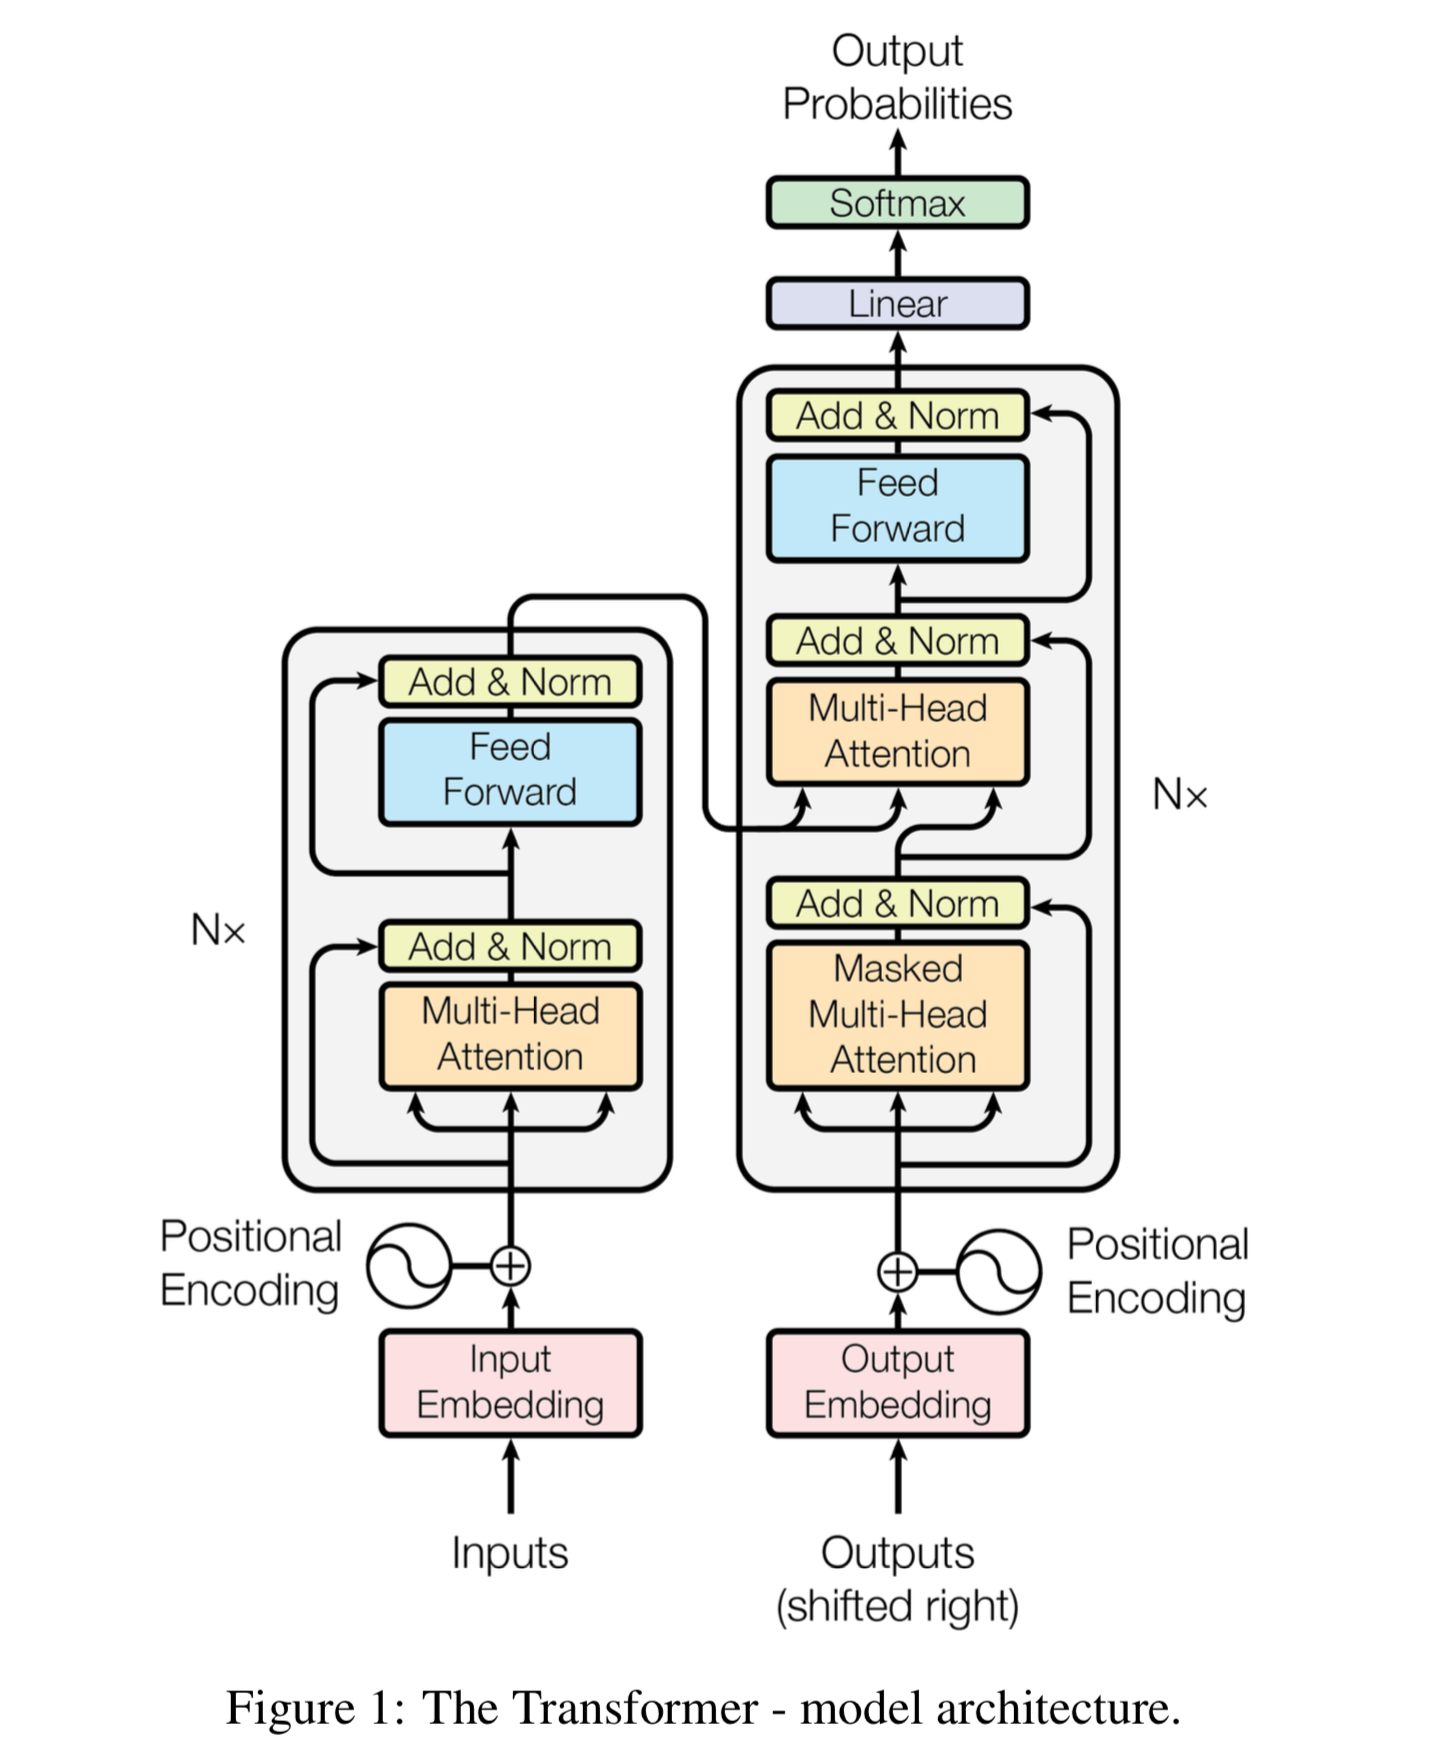
\includegraphics[width=0.6\textwidth]{image_model/model_transformers.png}
    \caption{Architecture de Transformers}
    \label{fig: Transformers} 
\end{figure}



On prend alors les données de textes qui sont une liste d'entiers, correspondant 
à l'indice de chaque mot du tokenizer de CamemBERT. Ces données passent alors dans CamemBERT, elles ressortent avec une dimension de
64. Elles passent alors dans une activation ReLU puis une couche dense de taille 64, puis une couche de dropout (avec un taux
d'oubli de $10\%$), pour enfin passer dans un dernier ReLU et une dernière couche dense à 2 dimensions. 
La Figure~\ref{fig: model_text} résume l'architecture de ce modèle, qu'on appelera \textit{TEXT}.

\begin{figure}[H]
    \centering
    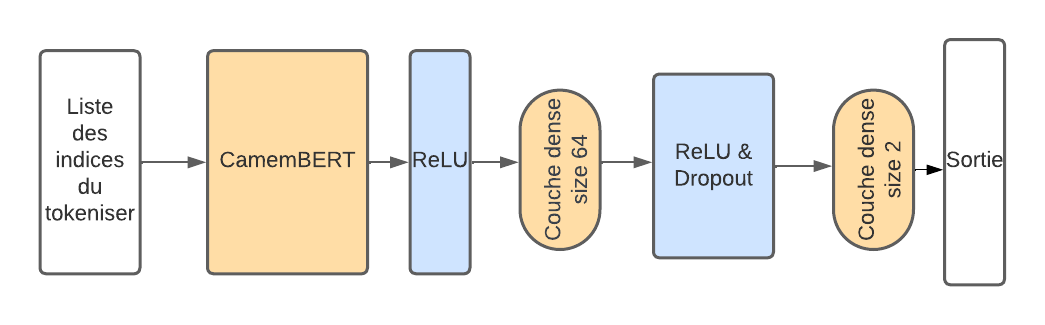
\includegraphics[width=0.7\textwidth]{image_model/model_text.png}
    \caption{Architecure du modèle \textit{TEXT}.}
    \label{fig: model_text}
\end{figure}

\subsection{Traitement de l'audio}

Afin de détecter les changements de parole dans des données audio, nous avons choisi d'exploiter une approche similaire en utilisant
un modèle avancé dans le domaine de la représentation audio : le modèle Wave2Vec~\cite{wav2vec}. Wave2Vec, basé sur les Transformers, s'est établi
comme une référence pour la tâche de traitement du signal audio, en particulier pour la détection des variations dans la parole.
Grâce à sa capacité à encoder de manière bidirectionnelle les représentations des signaux sonores, Wave2Vec excelle dans la
compréhension des nuances acoustiques et des transitions subtiles entre les locuteurs. 

On possède deux données en entrée qui sont les enregistrements audio des deux interlocuteurs. On fait alors passer leurs audio dans
Wave2Vec puis l'on concatène la sortie. On fait alors passer la concaténation dans une couche dense pour n'avoir qu'une sortie de
taille 2.
Eventuellement, ce modèle initial pouvait être amélioré en terme d'architecture, nous avons donc à l'issue de la concaténation,
ajouter une couche dense, puis une couche de ReLU et de dropout, et enfin finir sur une couche dense de sortie à 2 neurones. 
La Figure~\ref{fig: model_audio} résume l'architecture de ce modèle, qu'on appelera \textit{AUDIO}.

\begin{figure}[H]
    \centering
    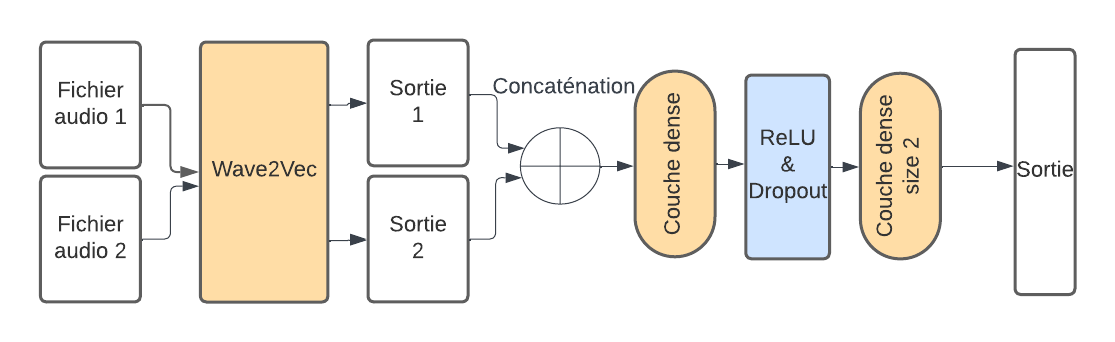
\includegraphics[width=0.7\textwidth]{image_model/model_audio.png}
    \caption{Architecure du modèle \textit{AUDIO}.}
    \label{fig: model_audio}
\end{figure}

\subsection{Traitement de la vidéo}

Pour traiter les données issues de la vidéo qui sont sous la forme des landmarks du visage des deux personnes en conversation,
nous avons choisi d'utiliser un réseau de neurones adapté à cette tâche d'analyse de séries temporelles : le réseau LSTM (Long-Short
Term Memory). En effet, ce modèle est pertinent pour la détection du changement de locuteur, car il est capable de conserver des
informations sur de longues séquences temporelles, ce qui est essentiel pour analyser les variations subtiles dans les mouvements
des landmarks faciaux. 

Comme pour l'audio, la vidéo contient un ensemble de deux fois 10 images pour chaque interlocuteur. On les fait alors passer
dans deux couches LSTM et on concatène les sorties pour ensuite les faire passer dans une couche ReLU et une couche dense de taille 2.
La Figure~\ref{fig: model_video} résume l'architecture de ce modèle, qu'on appelera \textit{VIDEO}.

\begin{figure}[H]
    \centering
    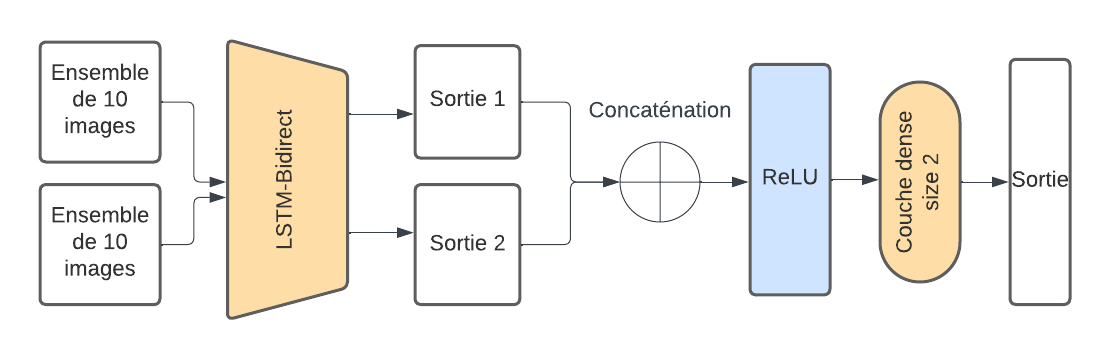
\includegraphics[width=0.7\textwidth]{image_model/model_video.png}
    \caption{Architecure du modèle \textit{VIDEO}.}
    \label{fig: model_video}
\end{figure}